The ability to perceive and reason about the world's actors, actions, objects, and relationships has been a longstanding goal for Computer Vision. Formally, we can benchmark progress towards this goal using tasks like Visual Question Answering, in which a model's reasoning skills are evaluated by it's ability to answer questions about visual stimuli. A variety of benchmarks have been created to test a model's capabilities at answering questions about images~\cite{johnson2017clevr,hudson2019gqa,antol2015vqa,zellers2019recognition,goyal2017making,krishna2017visual,zhu2016visual7w,kim2020answering} and about videos~\cite{tapaswi2016movieqa,lei2018tvqa,jang2017tgif,kim2017deepstory,xu2017video,maharaj2017dataset,zeng2016leveraging,yu2019activitynet, yi2019clevrer, mun2017marioqa}. Ideally, models trained on these benchmarks should be capable of reasoning over both spatial relationships between objects~\cite{krishna2017visual,lu2016visual} and temporal ordering of actions~\cite{zacks2001events,ji2020action}. Unfortunately, since most question-answering benchmarks operate over images, they are limited to only testing spatial relationships (e.g.~"What is on top of the table?")~\cite{hudson2019gqa,krishna2017visual,antol2015vqa} or at most guessing common sense events before and after the image \cite{park2020visualcomet}. The few existing video-only benchmarks have questions with simple temporal logic (e.g."What does the bear on right do after sitting?")~\cite{jang2017tgif,xu2017video,maharaj2017dataset,zeng2016leveraging,yu2019activitynet}, or are based on synthetically created videos in a constrained environment \cite{yi2019clevrer}. However, to answer questions that require models to jointly compose spatial and temporal reasoning in more complex questions (e.g."What did they do to the last object they put down before opening the window?"), we need newer benchmarks and a new class of models.

\begin{figure}[t]
    \centering
    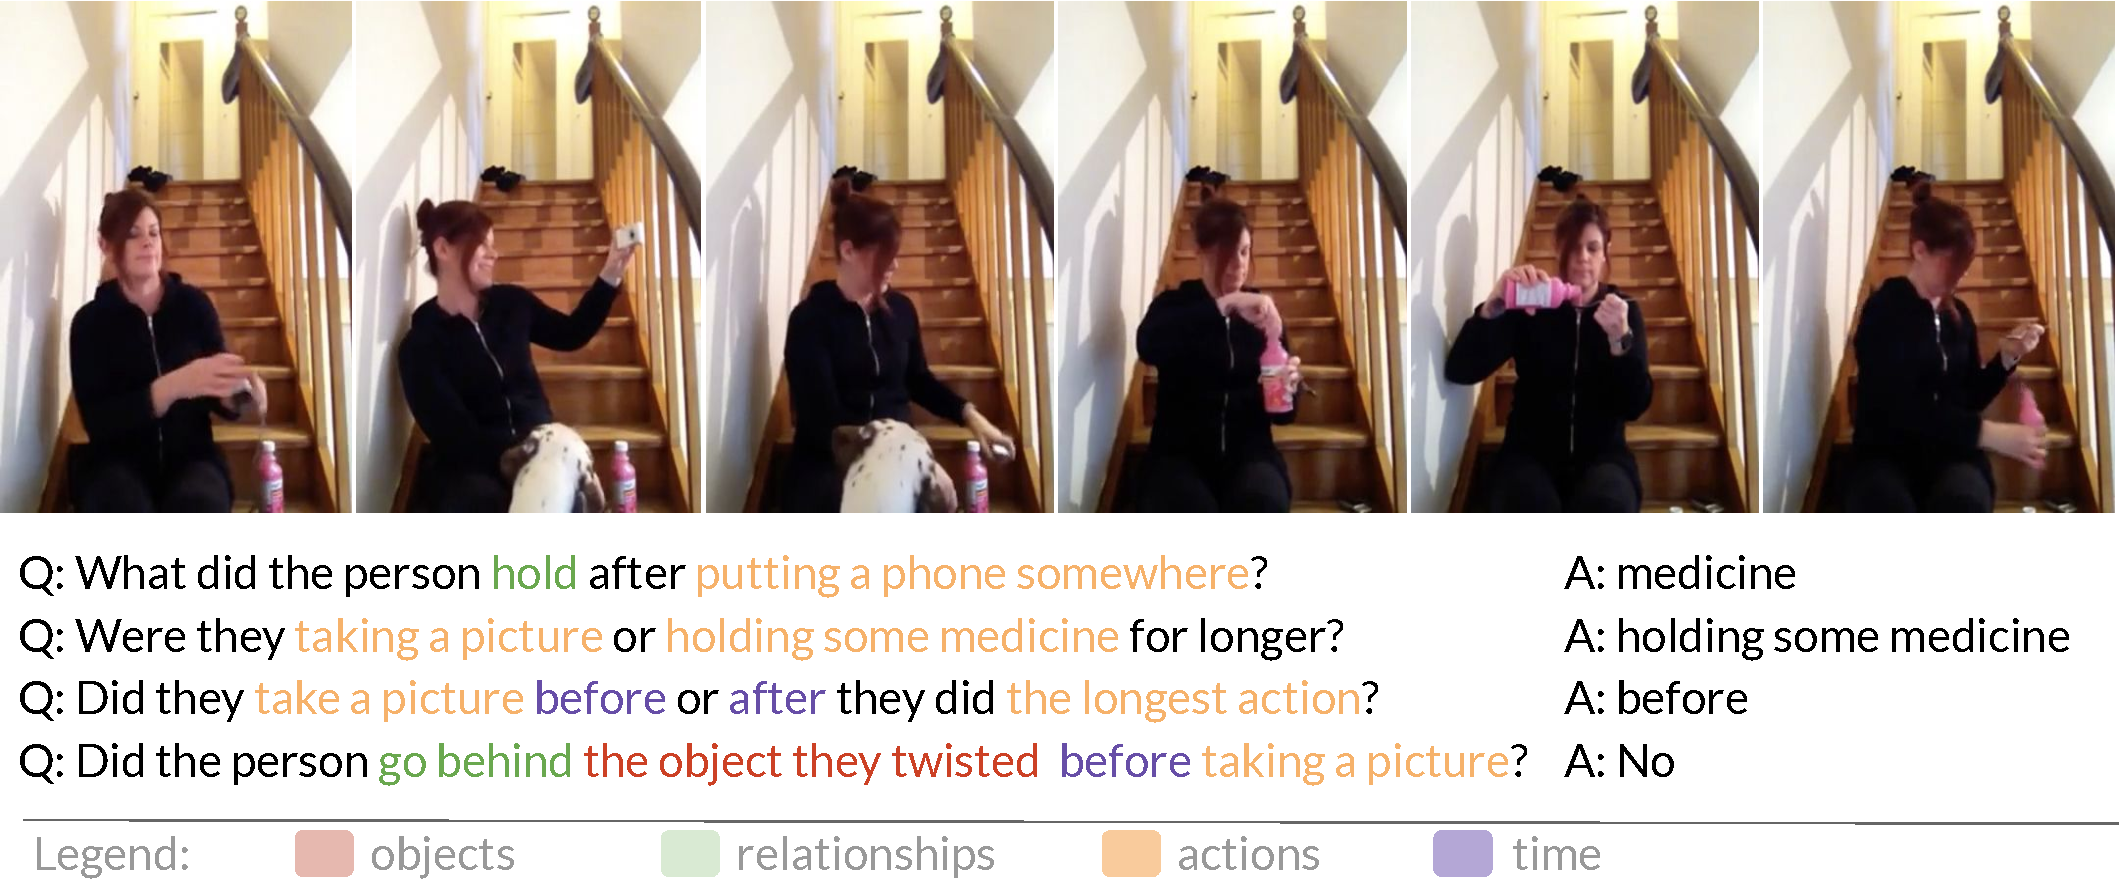
\includegraphics[width=\columnwidth]{figures/pull.pdf}
    \caption{TODO}
    \label{fig:pull}
\end{figure}

We introduce the Video Question Answering benchmark Action Genome Question Answering (AGQA) and use it to evaluate models on compositional spatio-temporal reasoning. AGQA measures a wider variety of spatio-temporal reasoning skills than existing benchmarks on real world \mgm{what is right terminology? natural videos? real world? non-synthetic?} videos, with balanced answer distributions for each question type. To achieve these goals, we developed \mgm{or built? or expanded upon? didn't necessarily develop} an automatic approach that converts Action Genome’s spatio-temporal scene graphs, containing objects, relationships, actors, and actions, into highly complex questions~\cite{ji2020action}. This process gives us tight control over the content of the questions to create a suite of metrics measuring individual spatio-temporal reasoning skills and compositional reasoning skills. 

Existing question-answering benchmarks are limited in the diversity of their questions. Since most benchmarks are image-based, they only test a model's reasoning over spatial relationships~\cite{johnson2017clevr,hudson2019gqa,antol2015vqa,goyal2017making,krishna2017visual,zhu2016visual7w}, object attributes~\cite{johnson2017clevr,hudson2019gqa, antol2015vqa,goyal2017making,krishna2017visual}, and common sense understanding~\cite{zellers2019recognition,antol2015vqa,krishna2017visual}. These benchmarks are unable to test reasoning over temporal relationships or activities beyond guessing based on common sense knowledge \cite{zellers2019recognition}. All questions asked by VideoQA benchmarks on non-synthetic videos that do not include extra textual information like dialogue limited temporal localization. Temporal localization refers to using the phrase "before/after/while $<$action$>$" to localize a relevant time in the video over which to reason. Questions in these benchmarks 1) can be answered from a single frame of the video, 2) apply to the entire video with no temporal localization, or 3) ask "what happened before/after/while $<$action$>$?"~\cite{jang2017tgif,xu2017video, maharaj2017dataset, zeng2016leveraging, yu2019activitynet}. Of the questions that apply to the entire video, some spatio-temporal topics are measured like counting and object and action recognition. 

Models should also be able to perform more complex temporal localization, follow the changing state of objects over time, sequence actions, and understand the concepts of action length, first, and last~\cite{lake2018generalization,vatashsky2020vqa}. Creating this diverse range of questions has previously been difficult. Questions automatically generated from video captions often lack diversity in structure~\cite{yu2019activitynet, jang2017tgif}, while human annotated datasets are too expensive to get a large enough sample to include a wide variety of categories~\cite{zeng2016leveraging, yu2019activitynet}. The community does not know how existing models perform on more complex temporal reasoning and generalization to new content because existing benchmarks do not have questions requiring these abilities. By recursively generating questions with direct references, indirect references, and temporal localizations, our question generation pipeline creates a diverse set of questions that can be trained and tested all together or separated by type.


Beyond measuring limited spatio-temporal reasoning, no existing benchmarks we know of measures a model's ability to generalize to new information. CLEVRER looks at compositional questions, but does not create metrics designed for measuring compositional reasoning \cite{yi2019clevrer}. Measuring models on compositional questions measures their ability to generalize from simple building blocks of information to more complex combinations. We adapt strategies from the constrained evaluation of the SCAN dataset \cite{lake2018generalization} to measure models' abilities to generalize to novel combinations of ideas, to adding temporal localizations and indirectly referencing ideas, to videos of longer lengths, and to more complex question structures.


We contribute a benchmark of XX complex question-answer pairs about Video inputs, and a suite of metrics to measure different spatio-temporal and compositional reasoning capabilities. We test AGQA on state-of-the art models to evaluate their strengths and weaknesses. 

%\mgm{Related work generally: I'm not sure how relevant all the parts are. CLEVR talks about how it balances answers and b/c its synthetic can do more in depth reasoning abilities. GQA talks about balancing answers and how CLEVR is synthetic, and other synthetic question generation methods. So i think focusing more of this section on the previous balancing attempts would help. I'm not sure how important the distinction between ImageQA and VideoQA is. Also neither of them split up the Related work into subsections.}